%!TeX encoding = UTF-8
%!TeX program = xelatex
\documentclass[notheorems, aspectratio=169]{beamer}
% aspectratio: 1610, 149, 54, 43(default), 32

\usepackage{latexsym}
\usepackage{amsmath,amssymb}
\usepackage{mathtools}
\usepackage{color,xcolor}
\usepackage{graphicx}
\usepackage{textcomp}
\usepackage{graphics}
\usepackage{textcomp}   
\usepackage{amsmath,amssymb}
\usepackage{array}
\usepackage{tabularx}
\usepackage{epstopdf}
\usepackage{picinpar}
\usepackage{verbatim}
\usepackage{subfig}
\usepackage{makeidx}
\usepackage{mathtools} 
\usepackage{pdfpages}
\usepackage{textcomp}
\usepackage{emptypage}
\usepackage[section]{placeins}
\usepackage{listings}
\usepackage{caption}
\usepackage{tikz}
\usepackage{tikz-3dplot}
\usetikzlibrary{patterns}
\usetikzlibrary{shadows,fadings}
\usetikzlibrary{positioning}
\usetikzlibrary{shapes.geometric}
\usetikzlibrary{arrows.meta,arrows}
\usepackage[toc,page]{appendix}
\usepackage{amsthm}
\usepackage{lmodern} % 解决 font warning
% \usepackage[UTF8]{ctex}
\usepackage{animate} % insert gif

\usepackage{lipsum} % To generate test text 
\usepackage{ulem} % 下划线,波浪线

\usepackage{listings} % display code on slides; don't forget [fragile] option after \begin{frame}

\usepackage{tcolorbox}
\usepackage{natbib}
\setcitestyle{authoryear}



% ----------------------------------------------
% tikx
\usepackage{framed}

\usepackage{pgf}
\usetikzlibrary{calc,trees,positioning,arrows,chains,shapes.geometric,%
    decorations.pathreplacing,decorations.pathmorphing,shapes,%
    matrix,shapes.symbols}
\pgfmathsetseed{1} % To have predictable results
% Define a background layer, in which the parchment shape is drawn
\pgfdeclarelayer{background}
\pgfsetlayers{background,main}

\definecolor{AmethystPurple}{HTML}{AEAEDF}
\definecolor{myblue}{RGB}{1,75,182}
% define styles for the normal border and the torn border
\tikzset{
  normal border/.style={black, decorate, 
     decoration={random steps, segment length=2.5cm, amplitude=.7mm}},
  torn border/.style={black, decorate, 
     decoration={random steps, segment length=.5cm, amplitude=1.7mm}}}

% Macro to draw the shape behind the text, when it fits completly in the
% page
\def\parchmentframe#1{
\tikz{
  \node[inner sep=1.5em] (A) {#1};  % Draw the text of the node
  \begin{pgfonlayer}{background}  % Draw the shape behind
  \fill[normal border] 
        (A.south east) -- (A.south west) -- 
        (A.north west) -- (A.north east) -- cycle;
  \end{pgfonlayer}}}

% Macro to draw the shape, when the text will continue in next page
\def\parchmentframetop#1{
\tikz{
  \node[inner sep=2em] (A) {#1};    % Draw the text of the node
  \begin{pgfonlayer}{background}    
  \fill[normal border]              % Draw the ``complete shape'' behind
        (A.south east) -- (A.south west) -- 
        (A.north west) -- (A.north east) -- cycle;
  \fill[torn border]                % Add the torn lower border
        ($(A.south east)-(0,.2)$) -- ($(A.south west)-(0,.2)$) -- 
        ($(A.south west)+(0,.2)$) -- ($(A.south east)+(0,.2)$) -- cycle;
  \end{pgfonlayer}}}

% Macro to draw the shape, when the text continues from previous page
\def\parchmentframebottom#1{
\tikz{
  \node[inner sep=2em] (A) {#1};   % Draw the text of the node
  \begin{pgfonlayer}{background}   
  \fill[normal border]             % Draw the ``complete shape'' behind
        (A.south east) -- (A.south west) -- 
        (A.north west) -- (A.north east) -- cycle;
  \fill[torn border]               % Add the torn upper border
        ($(A.north east)-(0,.2)$) -- ($(A.north west)-(0,.2)$) -- 
        ($(A.north west)+(0,.2)$) -- ($(A.north east)+(0,.2)$) -- cycle;
  \end{pgfonlayer}}}

% Macro to draw the shape, when both the text continues from previous page
% and it will continue in next page
\def\parchmentframemiddle#1{
\tikz{
  \node[inner sep=2em] (A) {#1};   % Draw the text of the node
  \begin{pgfonlayer}{background}   
  \fill[normal border]             % Draw the ``complete shape'' behind
        (A.south east) -- (A.south west) -- 
        (A.north west) -- (A.north east) -- cycle;
  \fill[torn border]               % Add the torn lower border
        ($(A.south east)-(0,.2)$) -- ($(A.south west)-(0,.2)$) -- 
        ($(A.south west)+(0,.2)$) -- ($(A.south east)+(0,.2)$) -- cycle;
  \fill[torn border]               % Add the torn upper border
        ($(A.north east)-(0,.2)$) -- ($(A.north west)-(0,.2)$) -- 
        ($(A.north west)+(0,.2)$) -- ($(A.north east)+(0,.2)$) -- cycle;
  \end{pgfonlayer}}}

% Define the environment which puts the frame
% In this case, the environment also accepts an argument with an optional
% title (which defaults to ``Example'', which is typeset in a box overlaid
% on the top border
\newenvironment{parchment}[1][Example]{%
  \def\FrameCommand{\parchmentframe}%
  \def\FirstFrameCommand{\parchmentframetop}%
  \def\LastFrameCommand{\parchmentframebottom}%
  \def\MidFrameCommand{\parchmentframemiddle}%
  \vskip\baselineskip
  \MakeFramed {\FrameRestore}
  \noindent\tikz\node[inner sep=1ex, draw=black!20,fill=black, 
          anchor=west, overlay] at (0em, 1em) {\sffamily#1};\par}%
{\endMakeFramed}

% ----------------------------------------------

\mode<presentation>{
    \usetheme{Warsaw}
    % Boadilla CambridgeUS
    % default Antibes Berlin Copenhagen
    % Madrid Montpelier Ilmenau Malmoe
    % Berkeley Singapore Warsaw
    \usecolortheme{orchid}
    % beetle, beaver, orchid, whale, dolphin
    \useoutertheme{infolines}
    % infolines miniframes shadow sidebar smoothbars smoothtree split tree
    \useinnertheme{circles}
    % circles, rectanges, rounded, inmargin
}
% 设置 block 颜色
\setbeamercolor{block title}{bg=black,fg=white}

\newcommand{\reditem}[1]{\setbeamercolor{item}{fg=red}\item #1}

% 缩放公式大小
\newcommand*{\Scale}[2][4]{\scalebox{#1}{\ensuremath{#2}}}

% 解决 font warning
\renewcommand\textbullet{\ensuremath{\bullet}}

% ---------------------------------------------------------------------
% flow chart
\tikzset{
    >=stealth',
    punktchain/.style={
        rectangle, 
        rounded corners, 
        % fill=black!10,
        draw=white, very thick,
        text width=6em,
        minimum height=2em, 
        text centered, 
        on chain
    },
    largepunktchain/.style={
        rectangle,
        rounded corners,
        draw=white, very thick,
        text width=10em,
        minimum height=2em,
        on chain
    },
    line/.style={draw, thick, <-},
    element/.style={
        tape,
        top color=white,
        bottom color=blue!50!black!60!,
        minimum width=6em,
        draw=blue!40!black!90, very thick,
        text width=6em, 
        minimum height=2em, 
        text centered, 
        on chain
    },
    every join/.style={->, thick,shorten >=1pt},
    decoration={brace},
    tuborg/.style={decorate},
    tubnode/.style={midway, right=2pt},
    font={\fontsize{10pt}{12}\selectfont},
}
% ---------------------------------------------------------------------

% Define colors similar to VSCode C++ syntax highlighting
\definecolor{vscodeblue}{rgb}{0, 0.27, 0.65}
\definecolor{vscodegreen}{rgb}{0, 0.5, 0}
\definecolor{vscodepurple}{rgb}{0.51, 0, 0.51}
\definecolor{vscodegray}{rgb}{0.3, 0.3, 0.3}
\definecolor{vscodeorange}{rgb}{0.8, 0.4, 0}
\definecolor{vscodecomment}{rgb}{0.47, 0.53, 0.6}
\definecolor{vscodestring}{rgb}{0.8, 0, 0}

% Set up the listings package for C++ code with VSCode-like coloring
\lstset{
  language=C++,
  basicstyle=\ttfamily\scriptsize,
  keywordstyle=\color{vscodeblue},
  commentstyle=\color{vscodecomment},
  stringstyle=\color{vscodestring},
  numberstyle=\tiny\color{vscodegray},
  identifierstyle=\color{black},
  emphstyle=\color{vscodeorange},
  frame=single,
  numbers=left,
  showstringspaces=false,
  breaklines=true,
  tabsize=2,
}


\lstdefinestyle{python}{
    language=Python,
    basicstyle=\ttfamily\scriptsize,
    keywordstyle=\color{blue},
    commentstyle=\color{green!60!black},
    stringstyle=\color{red},
    numbers=left,
    numberstyle=\tiny\color{gray},
    stepnumber=1,
    backgroundcolor=\color{white},
    frame=single,
    showspaces=false,
    showstringspaces=false,
    showtabs=false,
    tabsize=4,
    captionpos=b,
    breaklines=true,
    breakatwhitespace=false,
}
% ---------------------------------------------------------------------

%% preamble
\title[Diving into SPH]{Diving into SPH}
\author{Mustafa Bhotvawala}
\institute[]{}
\date{}
% -------------------------------------------------------------



\begin{document}

%% title frame
\begin{frame}
    \titlepage
\end{frame}


\section{SPH: What I've understood} 
\frame{\tableofcontents[currentsection]}

\subsection{Recap}

\begin{frame}[fragile]
  \frametitle{Navier-Stokes Equations}
  \framesubtitle{(Still N-S!)}
  
  The key idea is unchanged. You want to approximate the N-S equations as before, but not discretize your solution on a mesh. This is like any Lagrangian method. To recap the equations for continuum flow:
  
  \begin{itemize}
    \item Continuity Equation:
  \end{itemize}
  
  \[
  \frac{D\rho}{Dt} = -\rho \nabla \cdot \mathbf{u}
  \]
  
  \begin{itemize}
    \item Momentum Equation:
  \end{itemize}
  
  \[
  \frac{D\mathbf{u}}{Dt} = -\frac{1}{\rho}\nabla P + \nu\nabla^2\mathbf{u} + \mathbf{f}
  \]
  
  
  \end{frame}

  
\begin{frame}[fragile]
  \frametitle{Smoothed Particle Hydrodynamics (SPH)}
  \framesubtitle{What makes it different}
  
  \begin{itemize}
    \item SPH is mesh-free! Treatment of complex and/or moving geometries is easier
    \item Free surface flows that are challenging in Eulerian methods are more or less natural in SPH
    \item Exact (and simultaneous) conversion of mass and momentum
    \item Inherent parallelism
  \end{itemize}
  
  \end{frame}
  

  \subsection{Equations}

  \begin{frame}
    \frametitle{Kernels}
    \framesubtitle{Mathematical Form}

    In 3D and 4th order (also what I've used)
    \begin{equation}
      W(q) = \frac{21}{64\pi h^3} \cdot
      \begin{dcases}
        (2 - q)^4 (1 + 2q) & \text{if } 0 \leq q \leq 2 \\
        0 & \text{otherwise}
      \end{dcases}
      \end{equation}
    
    where:
    \begin{itemize}
      \item Kernels just convolve over the function, and aim to be an approximation to the Dirac Delta function
      \item It has compact support, which means the tail is not infitine, it takes a certain range of particles around it
      \item A kernel function must be consistent, i.e.:
    \end{itemize}

    \begin{equation}
      \int_{-\infty}^{\infty} W(q) \, dq = 1
      \end{equation}
    
    \end{frame}
    



  \begin{frame}[fragile]
  \frametitle{SPH Equations}
  \framesubtitle{Continuity}
  
  The approach in SPH is sto sum up contributions from neighbours.
  
  \begin{equation}
  \rho_a = \sum_{b} m_b \frac{W(\mathbf{r}_{ab}, h)}{\rho_b}
  \end{equation}
  
  % \begin{lstlisting}
  % rho[i] = sum_j(m[j] * W(r_ij, h) / rho[j])
  % \end{lstlisting}
  
  where:
  \begin{itemize}
    \item \( W \) is the smoothing kernel function.
    \item \( \mathbf{r}_{ab} \) is the vector from particle \( a \) to \( b \).
    \item \( h \) is the smoothing length.
  \end{itemize}
  
  \end{frame}



    \begin{frame}[fragile]
      \frametitle{SPH Equations}
      \framesubtitle{Momentum}
      
      The kernel functions can be differentiated - and this is used in the gradient for pressure in the momentum equation. Pressure is calculated from the equation of state. 
      
      \begin{equation}
      \frac{D\mathbf{v}_a}{Dt} = -\sum_b m_b \left( \frac{P_a}{\rho_a^2} + \frac{P_b}{\rho_b^2} \right) \nabla_a W_{ab}(h)
      + \nu \nabla^2 \mathbf{v}_a + \mathbf{f}_a
      \end{equation}
      
      where:
      \begin{itemize}

        \item \( P_a \) and \( P_b \), \( \rho_a \) and \( \rho_b \) are the pressures and densities of the current particle and its neighbours 
        \item \( \nabla_a W_{ab}(h) \) is the gradient of the smoothing kernel between particles \( a \) and \( b \) with smoothing length \( h \).
      \end{itemize}
      
      \end{frame}

      
      \section{Postprocessing} 
      \frame{\tableofcontents[currentsection]}

      \begin{frame}

      \frametitle{Numerical quantities}
      \framesubtitle{Kernel Weighted Interpolation}
      
      \begin{itemize}
       \item Postprocessing of SPH would involve interpolation of the same nature to obtain a numerical quantity from particle quantities
       \item We renormalize the interpolation using a Shepherd summation in the denominator
        \item  For instance, the numerical pressure \(P_a\) at particle \(a\) can be computed as a weighted sum of neighbour particles

       \[
        P_a = \frac{\sum_b P_b \frac{m_b}{\rho_b} W_{ab}}{\sum_b \frac{m_b}{\rho_b} W_{ab}}
        \]

      \end{itemize}

      \end{frame}


  \section{What I tried} 
  \frame{\tableofcontents[currentsection]}

  \subsection{A Simple Solver}
      
  \begin{frame}[fragile]
    \frametitle{A Simple Solver}
    \framesubtitle{Pressure Force}
    
    \begin{lstlisting}
      for(const auto& other : particles)
      {
        if(&p != &other)
        {
          double r = distance(p, other);
          if(r > 0)
          {
            double pj = calculatePressureTait(other);
            double rhoj = other.density;
  
            double w_press = wendlandGradient2D(r); 
  
            pressureForceX +=
              other.mass * (pi / (rhoi * rhoi) + pj / (rhoj * rhoj)) * w_press;
            pressureForceY +=
              other.mass * (pi / (rhoi * rhoi) + pj / (rhoj * rhoj)) * w_press;
          }
        }
      }
    \end{lstlisting}
    
    \end{frame}


    \begin{frame}[fragile]
      \frametitle{A Simple Solver}
      \framesubtitle{Density}
      
      \begin{lstlisting}
        double calculateDensity(const std::vector<Particle>& particles, const Particle& p)
        {
          double density = 0.0;
          for(const auto& other : particles)
          {
            double r = distance(p, other);
            density += other.mass * wendlandKernel2D(r);
          }
          return density;
        }
      \end{lstlisting}
      
      \end{frame}
      
    
      
      
    \begin{frame}[fragile]
    \frametitle{A Simple Solver}
    \framesubtitle{Main loop}
    
    \begin{lstlisting}
      for(auto& p : particles)
      {
          // From https://www.cs.cmu.edu/~scoros/cs15467-s16/lectures/11-fluids2.pdf
          p.vx += dt * p.fx / p.density;
          p.vy += dt * (p.fy / p.density - g); //add gravity here
          p.x += dt * p.vx;
          p.y += dt * p.vy;
          //recalculate forces in the next step
          p.fx = 0.0;
          p.fy = 0.0;
        }
        // Calculate density and pressure forces
        for(auto& p : particles)
        {
          p.density = calculateDensity(particles, p);
        }
        calculatePressureForce(particles);
        \end{lstlisting}
    
      \end{frame}

      \begin{frame}
        \frametitle{Just gravity}
        \framesubtitle{(Not much, but I'm glad I could get something basic up)}

        \begin{figure}
          \centering
          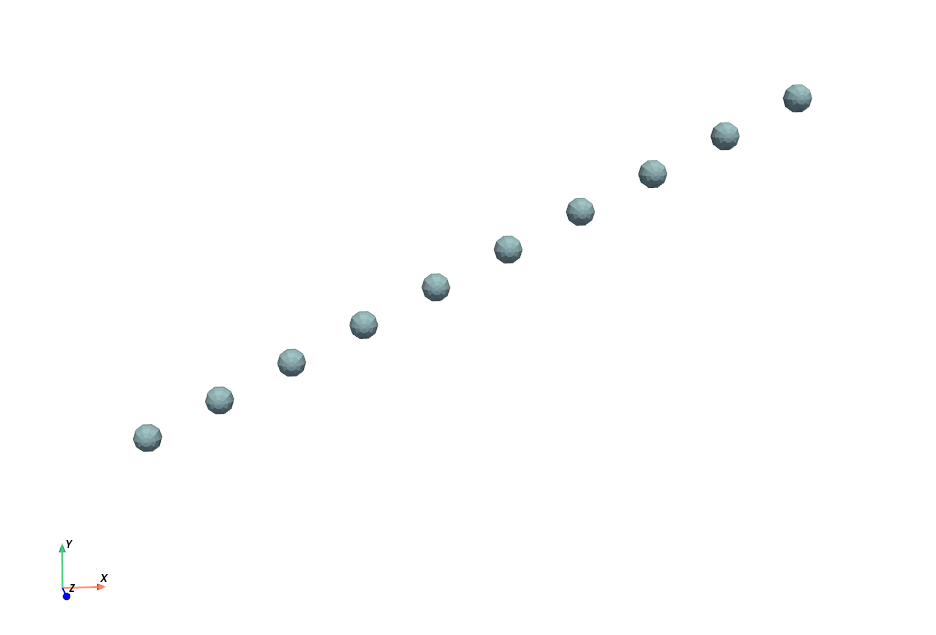
\includegraphics[width=0.5\linewidth]{pictures/solver_test.png} 
        \end{figure}
        
        *Using PyVista for this
      
      \end{frame}
      
  \subsection{Problem Statement}

  \begin{frame}
    \frametitle{Dam Break}
    \framesubtitle{PyVista Visualization}
    
    \begin{figure}
      \centering
      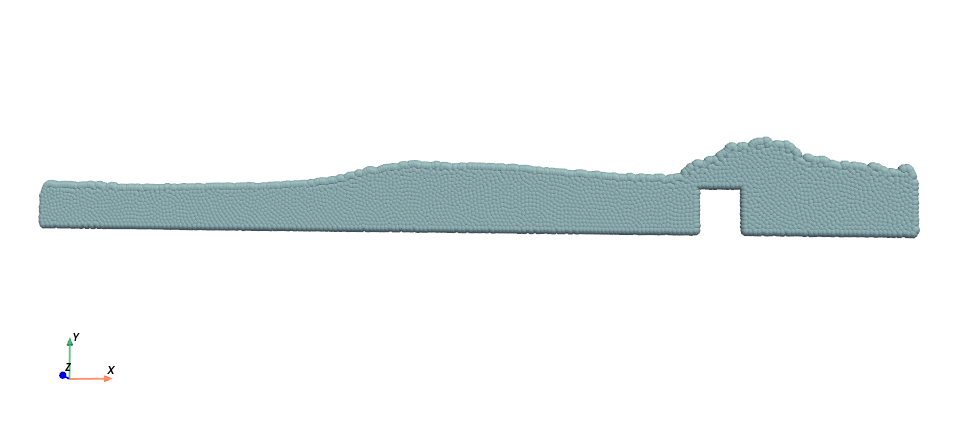
\includegraphics[width=0.8\linewidth]{pictures/domain_10000.png} 
      \caption{Domain at the end of the run}
    \end{figure}
  
  \end{frame}
 
  
  \begin{frame}[fragile]
    \frametitle{Dam Break}
    \framesubtitle{Generating CV Mesh}
    
    \begin{lstlisting}[style = python]
      def write_to_stl():
        x_resolution = 10
        y_resolution = 10
    
        x = np.linspace(0.07, 0.17, x_resolution)
        y = np.linspace(0.07, 0.17, y_resolution)
        z = np.zeros(1)  # 2D box, so z dimension has only one value
    
        grid = pv.RectilinearGrid()
        grid.x = x
        grid.y = y
        grid.z = z
    
        mesh = grid.cast_to_structured_grid().extract_surface()
        mesh.save("output.stl")
        mesh.plot("show_edges=True")
    \end{lstlisting}
    
  \end{frame}
  
  \begin{frame}

    
    \begin{figure}
      \centering
      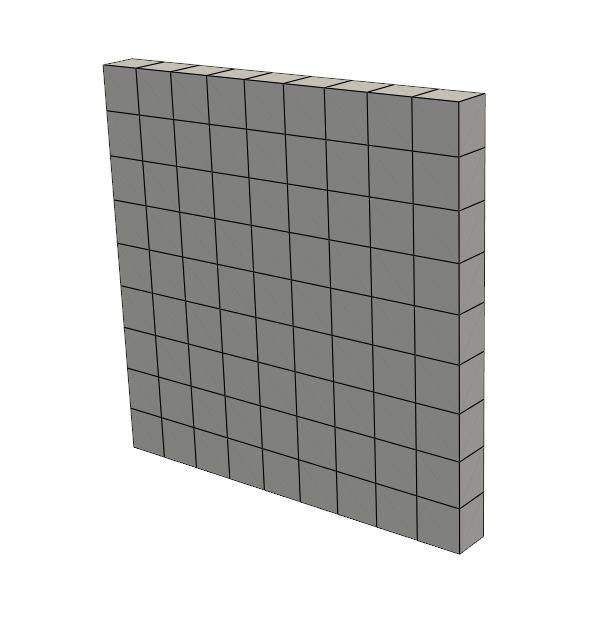
\includegraphics[width=0.4\linewidth]{pictures/control_volume_2.png} 
      \caption{Creating a control volume of the dimensions and location of the leftmost box}
    \end{figure}
  
  \end{frame}
  

  \begin{frame}[fragile]
    \frametitle{Dam Break}
    \framesubtitle{Recovering Surface Mesh in Nemo}
    
    \begin{lstlisting}[style = python]
    def read_into_nemo(): #note I could only read back an STL, so it's going to be triangulated..
        mesh =  n.Mesh.load(n.File("output.stl"))
        segmentcloud = mesh.data
        areas =  mesh.get_surface_area_per_segment()
        normals = segmentcloud.get_segment_normals()
  
      #  print(segmentcloud.point_attributes) #-->empty dict, how to proceed?
      #  print(segmentcloud.point_attributes["face_normal"])# KeyError: 'face_normal'
        
        #Riemann sum of a unit vector
        dot_product = np.sum(normals, axis=1) #horizontally sum across normals -> 1
        riemann_sum = np.sum(dot_product * areas)
      
        print('Riemann sum is:')
        print(mesh.get_surface_area())
        print(riemann_sum)
    \end{lstlisting}
    
  \end{frame}

  
  \begin{frame}

    
    \begin{figure}
      \centering
      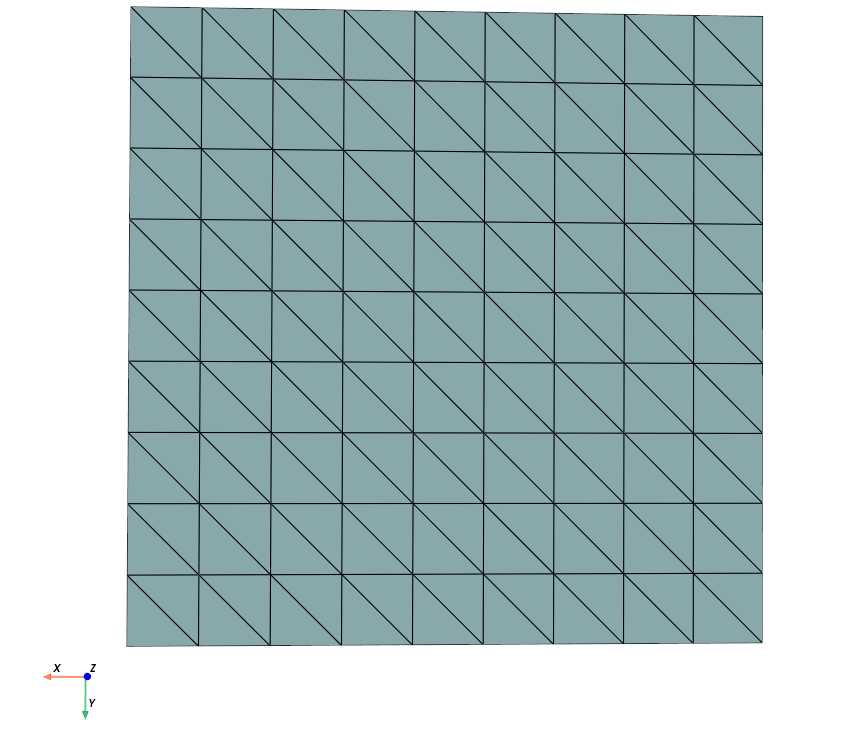
\includegraphics[width=0.5\linewidth]{pictures/control_volume.png} 
      \caption{Displaying the triangulated CV volume. Triangulated because I could only import back an STL and not a structured grid cast to a .vtu}
    \end{figure}
  
  \end{frame}
  
  \begin{frame}
    \frametitle{Interpolation}
    \framesubtitle{Control Volume}

    (I think the time was beyond the scope for me to implement this, but this is what I considered. This should apply to all quantities - flux and primitives alike)
    \begin{block}{Pseudoalgorithm}
      \begin{enumerate}
        \item Define a search radius = smoothing length $h$ for each particle (not sure, but could be a start)
        \item For each grid segment, look for neighbors within the radius $h$. Find atleast one point particle.
        \item Calculate value of numerical quantity using Shephard normalization and use value for grid segment. This is essentially a projection onto the cell centroid.
        \item Do Riemann sum over grid for total value on surface 
      \end{enumerate}
    \end{block}
  

  
  \end{frame}
  
  \end{document}